\subsection{Client zur Datenanalyse}

Der Client ist in Python implementiert, da zum Zeitpunkt, als die Probleme in der Adafruit BLE Library bekannt wurden, bereits große Teile des Clients implementiert waren. Zudem ist Python sehr leicht erlernbar und bietet gute Bibliotheken für eine Vielfalt von Anwendungsfällen.
\subsubsection{Graphisches User Interface}
Für die Darstellung graphischer Bedienelemente im Client, wurde die Library \texttt{PyQt4} verwendet, die eine leichte Integration der Graphen der Sensordaten ermöglicht. Diese werden mit Hilfe einer anderen Bibliothek erzeugt, können aber als ein sogenanntes Widget leicht in die GUI integriert werden.
Da keine Echtzeitübertragung der Daten möglich ist, werden nur wenige Bedienelemente, welche in einer Menuleiste untergebracht sind, benötigt:
\begin{itemize}
\item Öffnen einer Testdatei
\item Anzeigen von Statistiken über den Testlauf (Dauer des Testlaufs, gemessene minimal und maximal Werte)
\item Zusammenfügen von Dateien, wenn ein Testlauf in verschiedenen Dateien gespeichert ist
\item Parametrisieren und Anwenden des Filters
\end{itemize}
Werden vom Nutzer ungültige Eingaben gemacht, wird ihm dieser Fehler durch Dialogfenster mitgeteilt. 
\subsubsection{Datenformat}
Um alle weiteren Verarbeitungsschritte zu erleichtern wird ein einfaches Datenformat, welches Json ähnelt, verwendet. Die ausgelesenen Sensordaten werden in einem Tupel zusammen mit einem Zeitstempel, einer fortlaufenden Nummer und einer ID, welches den verwendenten Mikrocontroller identifiziert, gesendet.
\begin{figure}[h]
	\centering
	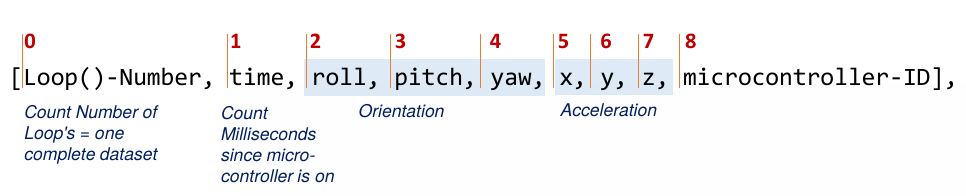
\includegraphics[width=1\textwidth]{images/k3-datenformat.png}
	\caption {Eingesetztes Datenformat}
	\label{fig:k3-datenformat.png} 
\end{figure}
\subsubsection{Parser}
Der Parser operiert auf oben beschriebenen Datenformat und hat zwei Hauptaufgaben:
\begin{itemize}
 \item Bereinigen der Daten, falls unvollständige, oder inkorrekte Tupel ankommen
 \item Aufteilen der Daten in Arrays, welche dann als Graph dargestellt werden können
\end{itemize}
Durch Eingabe einer Datendatei werden sechs Listen erzeugt, welche zur Darstellung and die Klasse \texttt{Plotter} übergeben werden. Die ersten drei Listen enthalten die Daten der drei Gyroskop Achsen, die letzen drei Listen die Daten der Achsen des Beschleunigungssensors. Da für die Werte der x-Achse die Zeitstempel verwendet werden, enthalten diese Listen jeweils Tupel der Form \texttt{(Zeitstempel, gemessener Wert)}.
\subsubsection{Darstellen von Daten}
Das Erzeugen der Graphen erfolgt in der Klasse \texttt{Plotter}, welche die Bibliotheken \texttt{numpy} und \texttt{pyqtgraph} verwendet. Für den Filter wird zudem noch die Bibliothek \texttt{scipy} benötigt. Durch \texttt{pyqtgraph} wird ein \texttt{PlotWidget} erzeugt, welches genau einen Graphen beinhaltet, der entweder die Werte der drei Achsen des Gyroskops oder des Beschleunigungssensors darstellt. Die y-Achse ist in der Einheit $\dfrac{\circ}{s}$ bei ersterem Graph und $\dfrac{m}{s^{2}}$ bei letzterem. Die x-Achse ist in beiden Graphen der Zeitstempel des Datentupels. (In \ref{fig:k3_4-graph.png} ist ein solcher Graph beispielhaft dargestellt).
\begin{figure}[h]
	\centering
	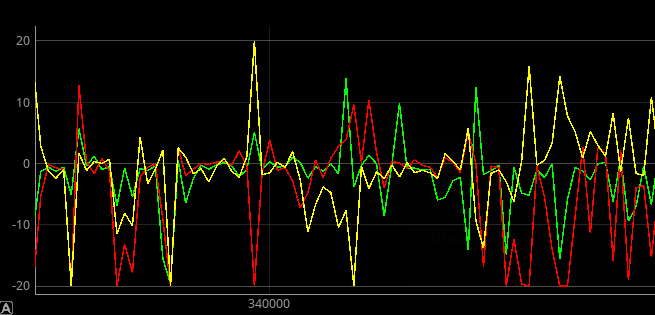
\includegraphics[width=0.75\textwidth]{images/k3-graph.png}
	\caption {Beispielgraph}
	\label{fig:k3_4-graph.png} 
\end{figure}
Ein \texttt{PlotWidget} enthält ein \texttt{PlotItem} welches eine Menge von \texttt{PlotDataItems} enthält, d.h. eine Menge von gemessenen Datenpunkten.
Für jeden der beiden Graphen wird dann in der Klasse \texttt{Presenter} eine Instanz der Klasse \texttt{Plotter} erzeugt und zu einer \texttt{QVBoxLayout} hinzugefügt. Diese dient dazu, die einzelnen enthaltenen Widgets relativ zueinander anzuordnen.
Damit die Graphen unabhängig der Anzahl der enthaltenen Datenpunkte gleichgroß dargestellt werden, wird die Größe des Fensters für jeden Graphen neu berechnet. Übersteigt die Größe des Graphen die Größe des Fensters, wird automatisch die horizontale Scrollbar angepasst.
\subsubsection{Datenaufbereitung}
Durch verschiedene äußere Bedingungen (z.B. Empfindlichkeit des Sensors oder Vibration der Bahn) werden die gemessenen Rohdaten verfälscht. Durch Anwendung von Filtern, können die Daten verbessert werden.
Hierbei wurden zwei Ansätze betrachtet, aber nur einer implementiert:
\begin{enumerate}
\item Savitzky-Golay-Filter
\item Kalman-Filter
\end{enumerate}
\paragraph{Savitzky-Golay-Filter}
Das Savitzky-Golay-Filter ist ein einfaches Glättungsfilter, bei dem auf die Daten der Kurve innerhalb eines Fensters eine polynomiale Regression angewandt wird. Das Filter hat gute Eigenschaften, wenn es um die relative Verteilung von Maxima und Minima geht. Es ist wahrscheinlich, dass durch die Empfindlichkeit der Sensoren bereits kleinste Vibrationen der Bahn aufgezeichnet werden. Diese geben jedoch kaum Aufschluss, in welchem Abschnitt der Sortieranlage sich das Schüttgut derzeit befindet. Größere Bewegungen, die auch in größeren Ausschlägen in den Sensoren resultiern, sind dafür besser geeignet. Insofern ist der Erhalt der Maxima und Minima von Nutzen.
Die Parameter, die bei diesem Filter verändert werden können, sind die Fensterbreite und der Grad des Polynoms. Je größer das Fenster und desto niedriger der Grad, desto mehr wird die Kurve effektiv gedämpft.
\paragraph{Kalman-Filter}
Das Kalman-Filter zieht im Gegensatz zum Savitzky-Golay-Filter zwei verschiedene Arten von Rauschen in betracht:
\begin{itemize}
\item Prozessrauschen 
\item Sensorrauschen
\end{itemize}
Jedoch ist die Wahl und Beschreibung des zu Grunde liegenden Systems entscheidend für die Parameterwahl. Ist das System nur unzureichend bekannt und wird deshalb schlecht beschrieben, ist der Filter nicht mehr als ein Tiefpass und wird keine guten Ergebnisse liefern. Da in unserem Fall die Erfahrung in der Anwendung eines solchen Filters fehlt, wurde dieser Ansatz bereits nach kurzer Zeit verworfen.\\
Die Wahl der Parameter ist beim Einsatz von Filtern entscheidend. Diese haben großen Einfluss auf die Form des resultierenden Graphen. Das macht sie aber auch besonders problematisch, da sie meist nur experimentell ermittelt werden können und unklar bleibt, wie weit die Graphen tatsächlich geglättet werden müssen, um ein verwertbares Ergebnis zu erhalten. 